\chapter{Dari Pembangkit Listrik ke Rumah: Alternator}\label{ch:g9:alternator}

\omterm{def:g9:electric-power-energy:kwh}{Kilowatt-jam} senilai setahun telah mengalir menembus pemeriksaanmu ---
tetapi dari mana? Ikutilah kabelnya keluar dari rumahnya, di bawah
jalannya, menyeberangi menara sutetnya, dan ia berakhir pada sebuah
mesin yang berputar di sebuah aula yang besar: \omterm{def:g9:alternator:alternator}{alternatornya}.
Rahasianya adalah kejutan yang terindah di dalam kelistrikan buku ini:
penemuan arus-membuat-kemagnetan tahun lalu, yang dijalankan terbalik.

\section{Induksi: efeknya dibalik}

\begin{proposition}[Induksi elektromagnetik]\label{prop:g9:alternator:induction}
Gerakkan sebuah \omterm{def:g1:magnets:magnet}{magnet} dekat sebuah \omterm{def:g3:first-electric-circuit:circuit}{rangkaian tertutup} --- atau
gerakkan rangkaiannya dekat \omterm{def:g1:magnets:magnet}{magnetnya} --- dan selagi geraknya
berlangsung, sebuah \omterm{def:g8:voltage-voltmeter:voltage}{tegangan} muncul lalu menggerakkan sebuah arus:
listrik yang \emph{diinduksikan} oleh kemagnetan yang berubah.
Aturannya, dari mejanya:
\begin{enumerate}
  \item hanya \emph{perubahan} yang menginduksikan: \omterm{def:g1:magnets:magnet}{magnet} yang diam
        di samping gulungannya, tidak ada apa-apa --- sekuat apa pun
        \omterm{def:g1:magnets:magnet}{magnetnya};
  \item gerak yang lebih cepat, \omterm{def:g1:magnets:magnet}{magnet} yang lebih kuat, lilitan
        gulungan yang lebih banyak: \omterm{def:g8:voltage-voltmeter:voltage}{tegangan} induksi yang lebih besar;
  \item baliklah geraknya, terbaliklah arus induksinya --- mendekat
        dan menjauh menggerakkan arak-arakan yang berlawanan.
\end{enumerate}
Tahun lalu sebuah arus membuat kemagnetan; tahun ini kemagnetan yang
bergerak membuat sebuah arus. Kedua efeknya adalah satu keping mata
uang, yang dibaca dari kedua wajahnya --- dan wajah yang kedua
menenagai peradaban.
\end{proposition}

\begin{method}[Induksi di atas meja]\label{met:g9:alternator:bench}
Sebuah gulungan berlilitan banyak, sebatang \omterm{def:g1:magnets:magnet}{magnet}, dan sebuah alat
ukur peka yang bernol di tengah:
\begin{enumerate}
  \item hubungkan alatnya melintang pada gulungannya; peganglah
        \omterm{def:g1:magnets:magnet}{magnetnya} diam di dalamnya: jarumnya tidur pada nol ---
        kekuatan saja tidak menginduksikan apa pun;
  \item sodokkan \omterm{def:g1:magnets:magnet}{magnetnya} masuk: jarumnya menendang ke satu arah ---
        lalu kembali ke nol pada saat geraknya berhenti;
  \item tariklah ia keluar: tendangan yang sama, ke arah yang lain;
  \item sodokkan lebih cepat: tendangan yang lebih besar. Goyangkan
        \omterm{def:g1:magnets:magnet}{magnetnya} masuk dan keluar dengan berirama, dan jarumnya
        berayun ke kiri, ke kanan, ke kiri --- kamu sedang memutar
        \omterm{def:g9:alternating-current:dcac}{arus bolak-balik} dengan tangan.
\end{enumerate}
\end{method}

\begin{omfigure}
\begin{tikzpicture}[scale=0.85]
  \draw[thick, fill=omThm, fill opacity=0.5]
    (0.4,1.2) rectangle (2.6,2.0);
  \node[font=\small] at (1.5,1.6) {U \quad S};
  \draw[-Stealth, very thick, omExo] (2.9,1.6) -- (4.0,1.6);
  \foreach \x in {4.4,4.8,...,6.8} {
    \draw[very thick, omDef] (\x,0.9) arc (200:340:0.32 and 0.75);
  }
  \draw[thick, omDef] (4.4,0.9) -- (4.1,0.2);
  \draw[thick, omDef] (7.4,0.9) -- (7.7,0.2);
  \draw[thick] (4.1,0.2) -- (4.1,-0.4) -- (5.2,-0.4);
  \draw[thick] (7.7,0.2) -- (7.7,-0.4) -- (6.1,-0.4);
  \draw[thick, fill=white] (5.65,-0.4) circle (0.45);
  \draw[-Stealth, very thick, omThm] (5.65,-0.4) -- ++(60:0.38);
  \node[right, font=\small] at (7.9,1.6)
    {sodok magnetnya: jarumnya menendang};
  \node[right, font=\small] at (7.9,1.0)
    {pegang ia diam: jarumnya tidur};
\end{tikzpicture}

{\small Induksi di atas meja: hanya \omterm{def:g1:magnets:magnet}{magnet} yang \emph{bergerak} yang
membangunkan gulungannya --- dan tendangan jarumnya terbalik bersama
geraknya.}
\end{omfigure}

\section{Alternatornya}

\begin{definition}[Alternator]\label{def:g9:alternator:alternator}
Sebuah \emph{alternator}\index{alternator} adalah induksi yang dibuat
tak kenal lelah: sebuah \omterm{def:g1:magnets:magnet}{magnet} yang diputar mantap di samping sebuah
gulungan yang terpancang (atau sebuah gulungan yang diputar di dalam
medan \omterm{def:g1:magnets:magnet}{magnet}). Tiap setengah putaran membawa sebuah kutub ke arah
gulungannya, lalu membawanya menjauh --- perubahan, yang diperbarui
tanpa henti --- sehingga \omterm{def:g8:voltage-voltmeter:voltage}{tegangan} induksinya berayun positif, negatif,
positif: \emph{bolak-balik}, menurut bangunannya, yang menggariskan
persis sinusoid yang mulus pada bab \omterm{met:g9:alternating-current:scope}{osiloskopnya}. Berputarlah lima
puluh putaran tiap sekon dan keluarannya berbolak-balik pada
\qty{50}{Hz}: \omterm{def:g8:sound-pitch-loudness:frequency}{frekuensi} jaringannya \emph{adalah} sebuah \omterm{def:g7:motion-average-speed:formula}{kelajuan}
putaran, yang dijaga selangkah oleh setiap pembangkit di jaringannya.
\end{definition}

\begin{example}[Dinamo di atas rodamu]\label{ex:g9:alternator:dynamo}
Dinamo sepeda adalah \omterm{def:g9:alternator:alternator}{alternator} sebesar saku: rodanya memutar sebuah
\omterm{def:g1:magnets:magnet}{magnet} kecil di dalam sebuah gulungan yang terpancang, dan lampunya pun
menyala --- lebih terang dan berfrekuensi lebih tinggi selagi kamu
mengayuh lebih keras, tepat sebagaimana dijanjikan aturan mejanya (dan
berkedip pada kayuhan yang merangkak, sebagaimana diamati bab
bolak-baliknya). Harganya jujur pula: dinamonya menyeret ---
menyalakan lampunya menuntut upaya yang sungguhan dari kakimu. Induksi
tidak memberi \omterm{def:g5:everyday-energy:energy}{energi}; ia \emph{mengubah} gerak menjadi listrik, \omterm{def:g9:kinetic-energy-safety:joule}{joule}
demi \omterm{def:g9:kinetic-energy-safety:joule}{joule}, dikurangi pajak gesekannya.
\end{example}

\begin{omfigure}
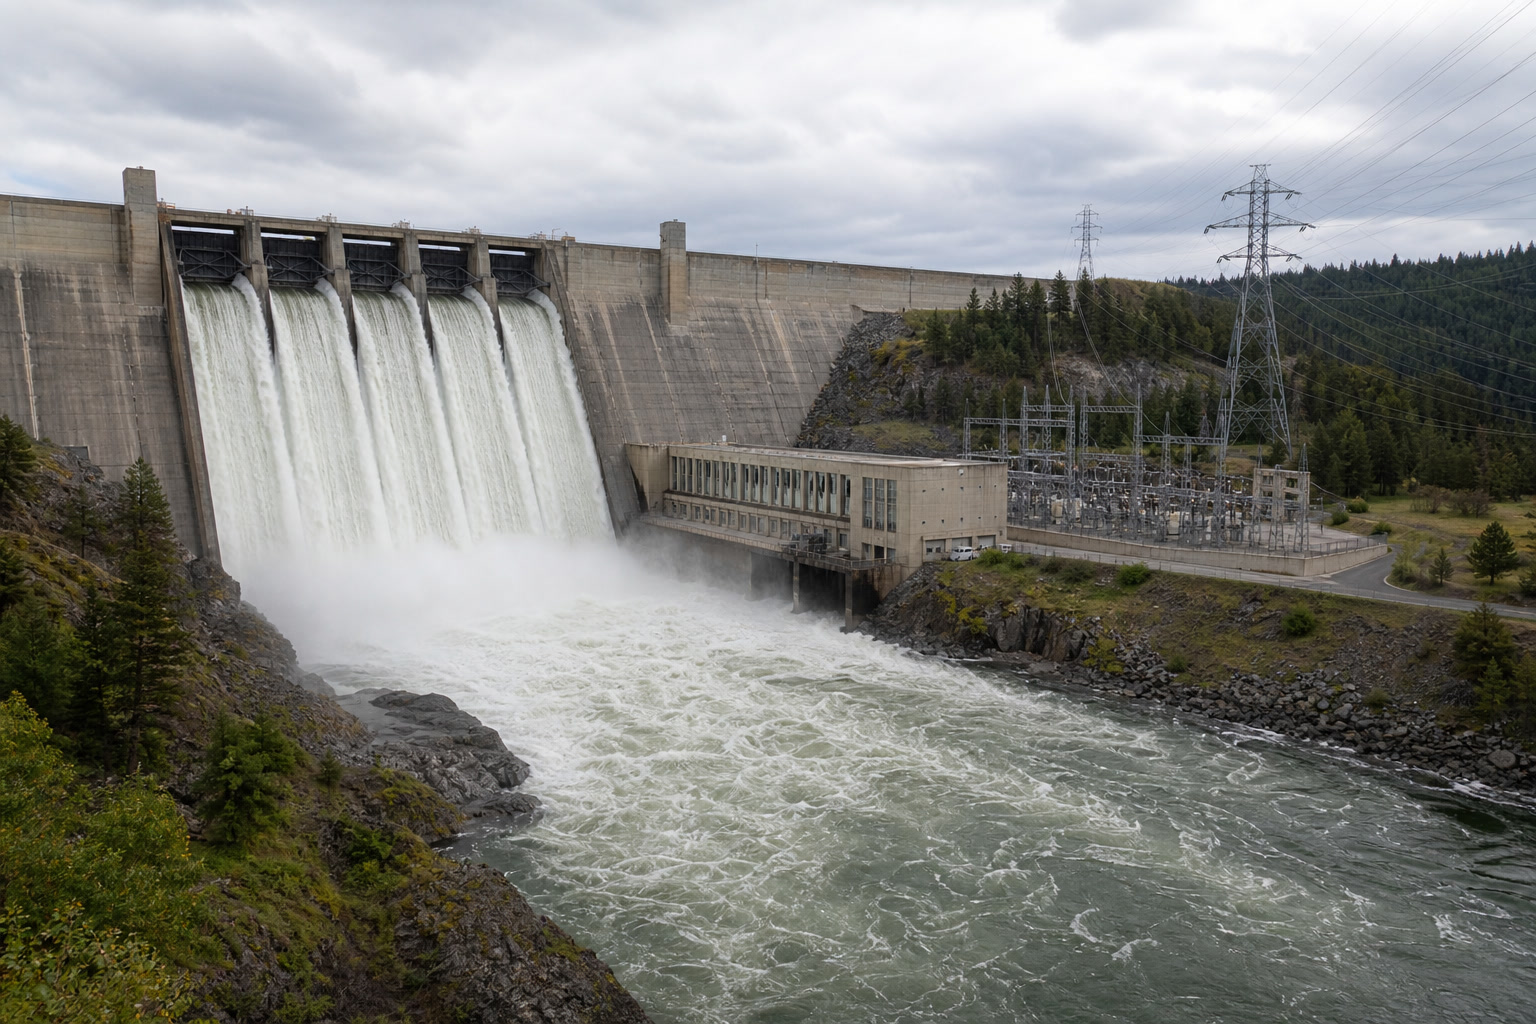
\includegraphics[width=0.55\linewidth]{images/book1/ai/g9-alternator-dam.jpg}

{\small Sebuah pembangkit listrik tenaga air: air yang terangkat menyerbu turun, memutar turbinnya, dan \omterm{def:g9:alternator:alternator}{alternatornya} mengirimkan \omterm{def:g5:everyday-energy:energy}{energinya} pergi di sepanjang kawatnya.}
\end{omfigure}

\section{Setiap pembangkit listrik adalah satu mesin}

\begin{proposition}[Inti yang sama]\label{prop:g9:alternator:core}
Boleh dikatakan seluruh listrik dunia, apa pun iklannya, dibuat dengan
cara yang sama: sesuatu memutar sebuah \emph{turbin} --- sebuah kincir
\omterm{def:g2:air-around-us:wind}{angin} bersudu yang kekar --- dan turbinnya memutar sebuah \omterm{def:g9:alternator:alternator}{alternator}.
Pembangkit listrik hanya berbeda dalam hal \emph{apa yang mendorong
sudunya}:
\begin{enumerate}
  \item pembangkit termal mendidihkan air dengan batu bara atau \omterm{def:g3:solids-liquids-gases:gas}{gas}
        yang terbakar --- semburan uapnya menggerakkan turbinnya;
  \item pembangkit nuklir justru mendidihkan airnya dengan \omterm{def:g5:heat-and-insulation:heat}{kalor} dari
        pembelahan atom --- uap lagi;
  \item bendungan listrik tenaga air membiarkan sebuah danau gunung
        jatuh menembus sudunya --- rantai bendungan masa kecilnya,
        yang dilengkapi;
  \item turbin \omterm{def:g2:air-around-us:wind}{angin} melewatkan perantaranya: anginlah dorongan
        sudunya, dengan sebuah \omterm{def:g9:alternator:alternator}{alternator} di dalam tiap rumah
        mesinnya.
\end{enumerate}
Satu kekecualian membuktikan aturannya: panel surya membuat listrik
sama sekali tanpa putaran --- lewat sebuah efek \omterm{def:g1:light-and-shadows:source}{cahaya} yang menjadi
milik tahun-tahun perguruan tinggi.
\end{proposition}

\begin{omfigure}
\begin{tikzpicture}[scale=0.8]
  \node[draw, thick, omExo, font=\footnotesize, align=center,
    minimum width=2.1cm, minimum height=0.95cm] (src) at (0.9,0)
    {nyala api, atom,\\danau atau angin};
  \node[draw, thick, omMeth, font=\footnotesize, align=center,
    minimum width=1.9cm, minimum height=0.95cm] (tur) at (3.8,0)
    {turbin\\(berputar!)};
  \node[draw, thick, omThm, font=\footnotesize, align=center,
    minimum width=2.0cm, minimum height=0.95cm] (alt) at (6.6,0)
    {alternator\\(induksi)};
  \node[draw, thick, omDef, font=\footnotesize, align=center,
    minimum width=2.0cm, minimum height=0.95cm] (gri) at (9.5,0)
    {trafo\\dan jaringan};
  \draw[-Stealth, very thick] (src) -- (tur);
  \draw[-Stealth, very thick] (tur) -- (alt);
  \draw[-Stealth, very thick] (alt) -- (gri);
  \node[below, font=\footnotesize] at (2.35,-0.75) {kalor atau gerak};
  \node[below, font=\footnotesize] at (5.2,-0.75) {putaran};
  \node[below, font=\footnotesize] at (8.05,-0.75)
    {arus bolak-balik};
\end{tikzpicture}

{\small Setiap pembangkit, satu rantai: sesuatu memutar turbinnya,
turbinnya memutar \omterm{def:g9:alternator:alternator}{alternatornya}, dan induksi melakukan sisanya. Hanya
kotak pertamanya yang berbeda dari pembangkit ke pembangkit.}
\end{omfigure}

\begin{example}[Rantainya, diperiksa]\label{ex:g9:alternator:chains}
Tuliskan tiap pembangkitnya sebagai rantai \omterm{def:g5:everyday-energy:energy}{energi} masa kecilnya, kini
dengan kosakata yang profesional. Bendungannya: simpanan tinggi $\to$
gerak air yang jatuh $\to$ putaran $\to$ listrik --- Matahari, ingatlah,
yang mengangkat danau itu lewat \omterm{def:g6:water-states:changes}{penguapan}: tenaga air adalah sinar
matahari yang ditangguhkan sebagai hujan. Pembangkit batu baranya:
simpanan kimia $\to$ \omterm{def:g5:heat-and-insulation:heat}{kalor} $\to$ gerak uapnya $\to$ putaran $\to$
listrik --- dengan kehangatan yang bocor pada setiap anak panahnya,
sebagaimana diakui bulu asap menara pendinginnya. \omterm{def:g2:air-around-us:wind}{Angin}: \omterm{def:g2:air-around-us:air}{udara} yang
bergerak (yang diaduk Matahari) langsung menjadi putaran. Sumber yang
diisi ulang alam --- air, \omterm{def:g2:air-around-us:wind}{angin}, \omterm{def:g1:light-and-shadows:source}{cahaya} matahari --- disebut
\emph{terbarukan}\index{terbarukan}; simpanan yang dibakar dan yang
dibelah habis untuk selamanya menurut skala waktu manusia.
\end{example}

\begin{remark}[Mengapa menara sutetnya berdengung pada 400000 volt]\label{rem:g9:alternator:transport}
Janji terakhir bab bolak-baliknya jatuh tempo. Sebuah kota memerlukan,
misalnya, seratus juta \omterm{def:g9:electric-power-energy:power}{watt}. Menurut $P = U I$, \omterm{def:g9:electric-power-energy:power}{daya} itu dapat
bepergian sebagai arus yang raksasa pada \omterm{def:g8:voltage-voltmeter:voltage}{tegangan} yang sederhana ---
atau arus yang sederhana pada \omterm{def:g8:voltage-voltmeter:voltage}{tegangan} yang raksasa. Tetapi kawat
memanas menurut \emph{arusnya} (\omterm{prop:g8:electric-current-effects:three}{efek panas} yang lama itu), dan setiap
derajat pemanasan menara sutetnya adalah \omterm{def:g5:everyday-energy:energy}{energi} berbayar yang hilang
kepada burung gagak. Karena itu jaringannya mengangkut pada \omterm{def:g8:voltage-voltmeter:voltage}{tegangan}
yang mendebarkan --- ratusan ribu \omterm{def:g8:voltage-voltmeter:voltage}{volt}, arus yang mungil, kehilangan
yang paling kecil --- lalu menurunkan \omterm{def:g8:voltage-voltmeter:voltage}{tegangannya}, lingkungan demi
lingkungan, sampai ke \qty{230}{V} yang jinak di dindingmu. Mesin
penurunnya, yaitu \emph{trafo}, adalah dua gulungan dan induksi sekali
lagi --- dan ia bekerja hanya pada arus yang berbolak-balik: seluruh
jaringannya berbicara AC karena trafonya berbicara AC.
\end{remark}

\section{Latihan}

\begin{exercise}[$\star$]\label{exo:g9:alternator:1}
Nyatakan ketiga aturan meja induksinya. Apa yang diinduksikan sebuah
\omterm{def:g1:magnets:magnet}{magnet} yang kuat \emph{ketika diam}?
\end{exercise}

\begin{exercise}[$\star$]\label{exo:g9:alternator:2}
Mengapa keluaran sebuah \omterm{def:g9:alternator:alternator}{alternator} berbolak-balik? Ikatkan perubahan
tandanya pada putarannya.
\end{exercise}

\begin{exercise}[$\star$]\label{exo:g9:alternator:3}
Pada \omterm{def:g7:motion-average-speed:formula}{kelajuan} putaran berapa sebuah \omterm{def:g9:alternator:alternator}{alternator} memberi makan jaringan
\qty{50}{Hz}? Karena itu apa yang harus disepakati setiap pembangkit
di jaringannya?
\end{exercise}

\begin{exercise}[$\star$]\label{exo:g9:alternator:4}
Sebutkan kedua kotak yang semesta pada setiap pembangkit listrik, dan
satu kotak yang berubah di antara batu bara, atom, bendungan, dan \omterm{def:g2:air-around-us:wind}{angin}.
\end{exercise}

\begin{exercise}[$\star$]\label{exo:g9:alternator:5}
Tuliskan rantai tenaga airnya dari danau gunung sampai ke lampumu ---
lalu sebutkan mesin langit yang mengisi danaunya.
\end{exercise}

\begin{exercise}[$\star$]\label{exo:g9:alternator:6}
Mengapa mengayuh menjadi lebih berat pada saat lampu dinamonya
menyala? Asas yang mana yang melarangnya menjadi lain daripada itu?
\end{exercise}

\begin{exercise}[$\star$]\label{exo:g9:alternator:7}
Pilahlah menjadi \omterm{ex:g9:alternator:chains}{terbarukan} dan bukan: \omterm{def:g2:air-around-us:wind}{angin}; batu bara; danau
bendungannya; uranium; \omterm{def:g1:light-and-shadows:source}{cahaya} matahari. Apa yang menentukan
pemilahannya?
\end{exercise}

\begin{exercise}[$\star$]\label{exo:g9:alternator:8}
Mengapa jaringannya mengirimkan \omterm{def:g9:electric-power-energy:power}{dayanya} pada ratusan ribu \omterm{def:g8:voltage-voltmeter:voltage}{volt}?
Sebutkan rumus yang menawarkan pilihannya dan efek yang memutuskannya.
\end{exercise}

\begin{exercise}[$\star\star$]\label{exo:g9:alternator:9}
Sebuah \omterm{def:g9:alternator:alternator}{alternator} peraga yang diputar tangan dengan lambat menyalakan
lampunya samar dengan kedipan yang terlihat; kalau diputar cepat,
terang dan mantap. Jelaskan kedua perubahannya dengan aturan mejanya
dan bab \omterm{def:g8:sound-pitch-loudness:frequency}{frekuensinya}.
\end{exercise}

\begin{exercise}[$\star\star$]\label{exo:g9:alternator:10}
Sebuah pembangkit mengantarkan \qty{1e8}{W}. Bandingkan arus yang
diperlukan pada \qty{230}{V} dan pada \qty{400000}{V} (dalam notasi
ilmiah). Yang mana yang dapat dibawa kabel yang sesungguhnya?
\end{exercise}

\begin{exercise}[$\star\star$]\label{exo:g9:alternator:11}
Pembangkit termal dan nuklir pada dasarnya adalah cerek yang rumit.
Belalah semboyan ini dengan rantainya --- lalu tentukan satu mata
rantai tempat keduanya berbeda.
\end{exercise}

\begin{exercise}[$\star\star\star$]\label{exo:g9:alternator:12}
Perjalanan besarnya, dijalankan terbalik: malam ini lampumu menyala
pada \qty{230}{V}. Telusurilah \omterm{def:g5:everyday-energy:energy}{energinya} ke hulu menembus setiap kotak
--- trafo, menara sutet, \omterm{def:g9:alternator:alternator}{alternator}, turbin, dan satu simpanan primer
pilihanmu --- sambil menyebut bentuk \omterm{def:g5:everyday-energy:energy}{energinya} pada tiap tahapnya dan
kebocorannya di sepanjang jalan. Lalu jawablah pertanyaan masa
kecilnya dengan kalimat kelas sembilan: dari mana pada akhirnya \omterm{def:g1:light-and-shadows:source}{cahaya}
di dalam kamarmu datang?
\end{exercise}

\section{Soal: Giliran Jaga Malam di Pembangkitnya}

\begin{problem}[{Soal akhir pekan --- giliran jaga malam di pembangkit
listrik tenaga air; induksi, selangkah, dan badainya; buku harian sang
insinyur}]\label{pb:g9:alternator:1}
Kamu membuntuti insinyur malam di bendungan lembahnya --- danau di
atas, kota di bawah, dan \omterm{def:g9:alternator:alternator}{alternator} yang berdengung di antaranya.

\medskip\noindent\textbf{Bagian I --- Aula mesinnya.}
\begin{enumerate}
  \item Insinyurnya membuka sebuah pintu air: airnya menggelegar
        menembus turbin tiga, dan alat ukur \omterm{def:g9:alternator:alternator}{alternatornya} pun bangun.
        Tuliskan rantai \omterm{def:g5:everyday-energy:energy}{energinya} dari danau ke rel \omterm{def:g9:electric-power-energy:power}{dayanya}.
  \item Di dalam \omterm{def:g9:alternator:alternator}{alternatornya}, apa yang bergerak dan apa yang tetap
        diam --- lalu mengapa sesuatu harus bergerak sama sekali?
  \item Jaringannya berjalan pada \qty{50}{Hz}. Insinyurnya
        memperhatikan sebuah papan ukur yang menjaga turbin tiga tepat
        pada putaran yang berpadanan. Apa yang salah pada \omterm{def:g7:motion-average-speed:formula}{kelajuan}
        yang keliru? (Apa yang akan dilakukan \omterm{def:g8:sound-pitch-loudness:frequency}{frekuensi} \omterm{def:g8:voltage-voltmeter:voltage}{tegangannya}?)
  \item Seorang murid magang bertanya apakah \omterm{def:g1:magnets:magnet}{magnet} yang lebih kuat di
        dalam rotornya akan memberi \omterm{def:g9:electric-power-energy:power}{daya} tambahan yang ``cuma-cuma''.
        Betulkan mimpinya dengan harga jujur milik dinamonya.
\end{enumerate}

\medskip\noindent\textbf{Bagian II --- Permintaan kotanya.}
\begin{enumerate}[resume]
  \item Pada pukul 03:00 kotanya menarik \qty{2e7}{W}. Pada
        \qty{200000}{V} milik jalur pengangkutannya, arus berapa yang
        meninggalkan pembangkitnya?
  \item \omterm{def:g9:electric-power-energy:power}{Daya} yang sama pada \qty{230}{V} akan memerlukan arus berapa
        --- dan apa yang dikatakan perbandingannya tentang tugas
        trafonya?
  \item Pada pukul 07:00, cerek dan pemanasnya bangun: permintaannya
        menggandakan diri. Insinyurnya harus memberi turbinnya lebih
        banyak apa, dan apa yang akan terjadi pada \omterm{def:g8:sound-pitch-loudness:frequency}{frekuensi}
        jaringannya kalau ia memberi terlalu sedikit? (Mesinnya
        melambat di bawah beban, seperti pengendara sepeda di sebuah
        bukit.)
  \item Pembangkit saudaranya --- sebuah ladang \omterm{def:g2:air-around-us:wind}{angin} di punggung
        bukit --- berhenti ikut ketika \omterm{def:g2:air-around-us:wind}{anginnya} mati. Kotak yang mana
        pada rantainya yang gagal, dan kotak yang mana yang berdiri
        sepenuhnya sehat?
\end{enumerate}

\medskip\noindent\textbf{Bagian III --- Badainya.}
\begin{enumerate}[resume]
  \item Petir memutus sebuah jalur pengangkutan; pemutus arusnya
        menjeplak. Insinyurnya mengalihkan \omterm{def:g9:electric-power-energy:power}{dayanya} lewat jalur
        tetangganya. Sifat jaringan yang mana --- satu jaringan
        paralel yang besar --- yang membuat pengalihannya mungkin?
  \item Selama kesibukannya, lampu sebuah gudang meredup kecokelatan
        selama semenit. Tafsirkanlah: apa yang melorot, dan \omterm{ex:g6:circuits-and-safety:motor}{motor}
        serta lampu gudangnya sejenak kekurangan apa?
  \item Fajar: buku hariannya harus menjelaskan kepada para murid
        magang mengapa listrik sepanjang malam itu, pada asalnya,
        berupa sinar matahari. Rancanglah penjelasan dua barisnya
        (danau, \omterm{def:g6:water-states:changes}{penguapan}, hujan).
  \item Baris terakhir buku hariannya, menurut kebiasaannya: fisika
        malam itu dalam satu kalimat --- dengan gerak, kemagnetan, dan
        cerek pagi kotanya di dalamnya.
\end{enumerate}
\end{problem}
